\documentclass[11pt]{article}
\usepackage{graphicx}
\usepackage{setspace}
\pagestyle{headings}
\linespread{1.6}

\begin{document}

\title{Hack All The History!: Working Title}
\author{Kevin Vilbig}
\date{Impending, Deadline, Get to work}
\maketitle

\begin{quote}
"There is only one time in the history of each planet when its inhabitants first wire up its innumerable parts to make one large machine...You and I are alive at this moment." 

\raggedleft{Kevin Kelly}
\end{quote}

Thanks to Richard Beyler for all of his guidance. Also thanks to Ann Marie Fallon, Lawrence Wheeler, Kathleen Merrow, Charles Baumbach, Mary Domski, and Lee Shaker for introducing me to the research skills and academic ideas that I needed to complete this project. There are many others who have helped me develop as a writer and a scholar over the years as well.

\begin{center}
This document was prepared with \LaTeX.
\end{center}

\newpage

\tableofcontents

\newpage

\section{Introduction}

What is a Hacker? All academics, regardless of discipline, turn first to Steven Levy’s 1984 writing\footnote{Levy, Steven. \emph{Hackers: Heroes of the Computer Revolution.} Durham: Anchor Press/Doubleday. 1984.} about the birth of this new culture. From the incubator on the ninth floor of an otherwise nondescript MIT edifice, this computational Utopia, this Eden of the machine god, a new culture was created, funded mostly by the advanced defense research wing of the Department of Defense, DARPA\footnote{cite Abbate}. The ethical basis of this culture was in stark contrast to Cold War America. 

[Insert paragraph blah blah blah cold war America]

Not to mention MIT’s institutional requirements for entry. It takes a massive leap of propaganda in order to imagine an anarchistic, Edenic, computational utopia flourishing in that kind of institutional environment. If anything, we should characterize this space as a monastary, complete with (presumably) celibate monks supplicating to the sanctuary of the one-true machine-god, living a relatively simple life, with the all consuming goal of contemplation of, and periodic communion with, the machine. If the Hacker Ethic was a product of artificial institutional construction, is it universally applicable outside of those artificial, institutional boundaries?

Levy Itemizes The Tenets of the Hacker Ethic in Chapter 2:
\begin{itemize}
\item Access to computers -- and anything which might teach you something about the way the world works -- should be unlimited and total. Always yield to the Hands-On Imperative!
\item All information should be free
\item Mistrust authority -- promote decentralization
\item Hackers should be judged by their hacking, not criteria such as degrees, age, race, sex, or position
\item You can create art and beauty on a computer
\item Computers can change your life for the better
\end{itemize}

Also, we need to discuss about the complex evolutionary process of identity with regard to hackers. These days, technicaly minded students are faced with a dizzying array of specializations and sub-specializations related to computer science and electrical engineering. Do you want to be a Software Engineer, Computer Engineer, Electrical Engineer, Computer Scientist, Telecommunications Engineer, Electronics Engineer, etc? It turns out there are a multitude of government, military, and industrial agents that are driving the creation of these programs in order to train students for certian career potitions that they already have mapped out. It's like an easy assembly line for training workers and soldiers. Just step into this line here, and four years later you'll come out a fully certified professional. Where do the hackers fit into this institutional system? As often as not, they were dropouts, miscreants, and troublemakers as far as the instutitional systems were concerned. They're seen as abberations, geniuses, troublemakers, or as we've seen with the recent tragedy in Aaron Swartz's death, criminals. Bill Gates is a notable Harvard dropout, and is merely a singular example of a much wider trend throughout hackerdom.

I assert that the evolution of the Hacker Ethic had more to do with institutional and political factors than purely scientific or even hackerific goals\footnote{This isn't really different from the development of any other Intellectual Revolution, cite something here, I forget what}. [The environmental pressure that drove the alteration of this idea over time was the influence of the dominant culture?] My intent is to isolate the expression of the Hacker Ethic in the various periods of the Computer Revolution from 1959 - 1991, ending this historical narrative with the release of Linux 0.1. These periods are divided up into the gestation of the culture in MIT, it’s ensuing spread to Stanford and other universities during the 1960s. At the same time, the phreaks were playing around with the telephone system. Then, the 1970s saw the rise of the personal computer, with the Silicon Valley being the Mecca of the microchip. Then the explosion of mechanized digitized communication leads to the Hacker Ethic being transmitted via the BBS community in the 80s and then, it was popularly expressed via the Hacking and Phone Phreaking scenes and the development of the Free and Open Source Software (FOSS) principles that guide the movement to this day. The Hacker Ethic was created by the 60s counterculture, for the counterculture, and then it spread underground through the BBS systems and ARPAnet and constantly clashed on a large scale with the dominant millieu of Intellectual Property, Copyright, etc. The Hacker Ethic may also be characterized as a sort of ideal agent-provocateur, since it was birthed and weaned on the dime of the DoD.

\section{A Story in Parts}

In order to reasonably discuss Hackers and History in the same project, we must first anchor this strange phenomenon of a Hacker into the greater sweep of the History of information. I can't possibly encompass the whole of human history in this meager paper. When I first started thinking about this I became tempted here to expand the definition of information transmission to include everything from smoke signals and mountain top signal fires, to Florentine ciphers during the Renaissance, to American Revolutionary pamphlets, but I can't explore that and still be able to encounter the focus of this project, the Hackers. 1959 - 1991 are the years of interest. 1959 marks the first encounter of the MIT Tech Model Railroad Club's signals division with the TX-0 in the second floor of MIT's Building 26. 1991 is the year when Linus Torvalds released the 0.1 Alpha of his now famous operating system, Linux. I think that by limiting the scope of this project to that range, I will avoid having to discuss the explosion of the consumer internet in the 1990's.

\begin{figure}[ht!]
\center
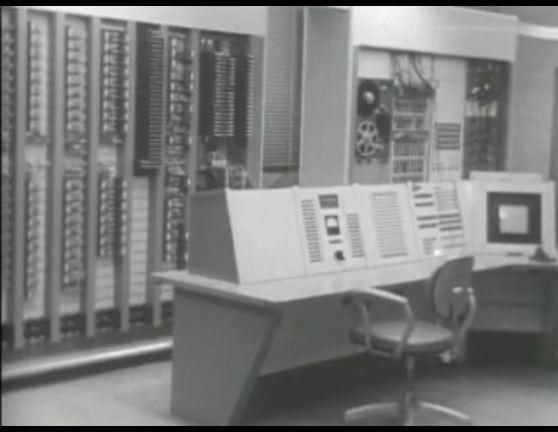
\includegraphics[width=80mm]{TX-0.jpg}
\caption{The TX-0: screenshot from MIT CSAIL video Archive http://www.csail.mit.edu/videoarchive/history/aifilms/museum-105}
\end{figure}

The story of this culture is intertwined with some key advances in technology. I am going to briefly trace the advances of the total history of human communication technology. From smoke signals, to mountaintop signal fires, to the mechanical printing press, to electric wires transmitting binary codes for the telegraph, to the first transatlantic radio transmissions with a spark-gap generator, and onward through coherent lasers -- transmitting data through fibers of spun glass. I avoid giving the nearly mythological stories in Levy’s journalistic chronicle the genetic weight in this story.  I would like to follow other historians of technology by inserting first networked computer systems as nothing more than another step along this track of transmitting binary data, whether via smoke signals or electric pulses, as no less than humans using tools to transmit data to other humans. Daniel Headrick has already done a lot of this work for me through the age of Imperialism. And Janet Abbate also informs the discussion about the institutional pressures that created the ARPAnet. The coevolution of the network of BBS systems that piggybacked on top of this Imperially constructed telecommunications system, built alongside and finally interconnected with the ARPAnet, became what we see as the internet today.\footnote{BBS} Most of the cultural norms and values (like the Hacker Ethic) that we see emerge from the Internet were not necessarily born on the ARPAnet mainframe systems. This culture was built in the interaction of computers attached to the telephone network, being used, not for it’s popular purpose of sending single voice communications, but instead being used to transmit computer data using MODEMs and hobbyist microcomputer systems.

This couldn't have been accomplished without the Silicon Valley 

Every Golden Age ends in a fall from grace. I will also be tracing the codification of the criminality of hackers to a single document released in 1982 by the Department of Justice, Bureau of Justice Statistics.  It outlines exactly what a computer crime is. Amusingly, it heralds the “Dawn of the Age of Aquarius” to usher in the “Age of the Computer” (quoted this, I can’t make this shit up). Hackerdom has, by now, eaten from the fruit from the tree of knowledge of good and evil.\footnote{The first Apple computer's retail price was \$666.66 afterall.}  Thus begins the fall. By the time this story ends, the mythological teenage hacker becomes public enemy number one. \footnote{Is your son (of course) up in his room, breaking into FBI databases and committing bank fraud? News @ 11.} Highly coodrinated and even more highly publicized, the FBI busts rings of hackers all over the country\footnote{Sterling, Bruce. \emph{The Hacker Crackdown}. } This was the next stage in the expansion of the hacker culture. I will be looking at a wide selections of texts that look at these new kinds of hackers, phreaks, and crackers, and the scene spreads to the streets. There are a dozen books written about the topic that are compiled from literally hundreds of news articles\footnote{Cite all the books!}. I will also be looking at popular underground magazines from this era, Phrack, 2600, as well as exploring some popular hacker archives of BBS material. I will also be looking at other primary source material from this era in order to trace the evolution of hackerdom through it’s clashes with the dominant culture in America as well as the government’s systematic involvement in enforcing and enabling computer security after, if accidently, creating the culture of free exploration so touted from the Golden Age.

Then we come to the next major milestone in the development of this culture, with convergent ideational evolution, the GNU project and Linux both come together to form a fully functioning operating system that has been likened to giving away fully functional M1-A1 Abrams tanks by lining them on the side of the road with the keys in the ignition. (In the beginning was the command line, Neal Stephenson, a footnote about the popular automotive metaphor for computer programs might be fun here. Now, here we need to explore the ideas of both, ideas evolving as an ecosystem, hybridizing, breeding, growing, and some dying out. And, we also need to explore the idea of convergent evolution. As it so happens, like Newton and Leibniz both seem to have independently invented the mathematical ideas that we so rudely codify into Calculus textbooks, many of these ideas were developed by different people in different places, independent of the other. So should that be a race to the patent office? Who gets the global rights to an algorithm that is probably actually already in some dead mathematician’s notes? This is a can of worms that I will not be opening in this paper, except maybe to get a little whiff of the problem. It doesn’t smell very appetizing, but it will be necessary to settle the IP debate in the future. (I will look into Mario Biagioli’s work here to see what he’s been up to)

The final part of this evolution is still happening right now. It happening at hacker conferences all over the world, in every country, on every continent, every month, every day in hackerspaces, every time somebody openly commits a patch to the linux kernel, or submits a bug report to firefox. There are more projects than I have space to explore in the scope of this project. The important thing about the final part of this evolution is that the core ethic of sharing software, legitimized by the mythology of the Golden Age, is expanding outside of that narrow realm of algorithms and software. Wikipedia, Open Source textbook initiative in California just passed, the RFHack open source hardware (funded by the same DARPA that built the Golden Age), Ethiopian children hacking OLPC’s with no outside guidance. It’s not just about software anymore, and it’s not just about sharing with the small Utopian group in a constructed environment.



\section{Common Evidence,  Divergent Methodology}

Hackers are a scholarly topic in vogue for the past decade or so, though they have a relatively long history as academic targets. Joseph Weizenbaum was a professor at MIT during the inception of the first TMRC Hackers who coined the term and codified much of the jargon that is still in use today. He dedicated a chapter of his 1976 text to a diatribe against the most passionate of the TMRC hackers.\footnote{Weizenbaum, Joseph. "Science and the compulsive programmer." \emph{Computer Power and Human Reason.} San Fransisco: W.H. Freeman and Company. 1976.} There has also been scholars from all over the spectrum of academia sticking their noses into Hackerdom. Anthropologists\footnote{Kelty, Chris. \emph{Two Bits.} and Coleman, Gabriella \emph{Coding Freedom.}}, Business, Marketing, Political Science, Criminoligists, Philosophers, and more. The common texts that are cited again and again include Levy's \emph{Hackers: Heroes of the Computer Revolution}. Like \emph{Burckhardt's Civilization of the Renaissance in Italy,} this truly is the seminal work. Though the comparison falls apart when we start to think about the relative temporal distance between the texts and their subjects, as Levy was able to directly interview many of the people involved. How much distance do we need to have from a historical subject in order to study it as history? If Thucydidies is considered the first historian, then couldn't Levy be, also? Regardless, you can't discuss hackers without this 1984 text. Most of the scholars also give a cite to Richard Stallman's essays on Free Software, as well. They also turn to Eric S. Raymond's \emph{Cathedral and the Bazaar.} as another key text to explain just what makes this whole phenomenon tick. Raymond is also known for publishing the Jargon File as The New Hacker's Dictionary, a bright yellow tome filled with almost as many amusing cartoons as useful definitions. It's chock full of tongue in geek humor about dealing with the craziness of networked computer systems in Universities.

I am going to be doing a semiotic exploration of the artifacts that emerged from the birth of this culture.\footnote{Coleman. 6.} My primary source material will include the popular zines, 2600:The Hacker Quarterly and Phrack magazine, both started in 1984. I am also looking at copies of earlier computer magazines, Byte and Creative Computing. I also am going to be digging into some of the Homebrew Computer Club's newsletters. There are some other interesting bits and pieces that I will share when I get to that part, but that's the meat of it. I am specifically filtering out the meat of the technical articles and looking for things that suggest the philosophical and political motivations of the publishers regarding this Hacker Ethic. I'm sifting through these archives relatively quickly. So, this will not be an exhaustive exploration at this point, but more a collection of snapshots over time that show the evolution of this idea as the pressures from the outside world, economics, government, and bluntly, power, effect the ideas and methods of these groups of people. As the networks began to turn into a massive Command and Control network for militaries across the world, and into logistics mechanisms for the military industrial complex, the fears of the original Berkeley protestors who wore punchcards around their necks became more realized than they would ever imagine. The world of today, where your name and face are run through computers every day for facial recognition, employment verification, credit, financial transactions. It's almost sickenly poetic that 1984 was the year that these magazines all started reporting. Orwell may have overestimated the impact and pace with which Big Brother's watchful eyes peer down on society, but his ominous vision is a part of the society we are living in today.
\begin{singlespace}
\noindent I like to think (and\\
the sooner the better!)\\
of a cybernetic meadow\\
where mammals and computers\\
live together in mutually\\
programming harmony\\
like pure water\\
touching clear sky.\\

\noindent I like to think\\
\indent (right now, please!)\\
of a cybernetic forest\\
filled with pines and electronics\\
where deer stroll peacefully\\
past computers\\
as if they were flowers\\
with spinning blossoms. \\

\noindent I like to think\\
\indent (it has to be!)\\
of a cybernetic ecology\\
where we are free of our labors\\
and joined back to nature,\\
returned to our mammal\\
brothers and sisters,\\
and all watched over\\
by machines of loving grace.\footnote{Brautigan, Richard. "All Watched Over by Machines of Loving Grace". San Francisco. The Communication Company. 1967. Print. }
\end{singlespace}


\section{Clay Tablets and Telegraphs?}


\begin{figure}[ht!]
\center
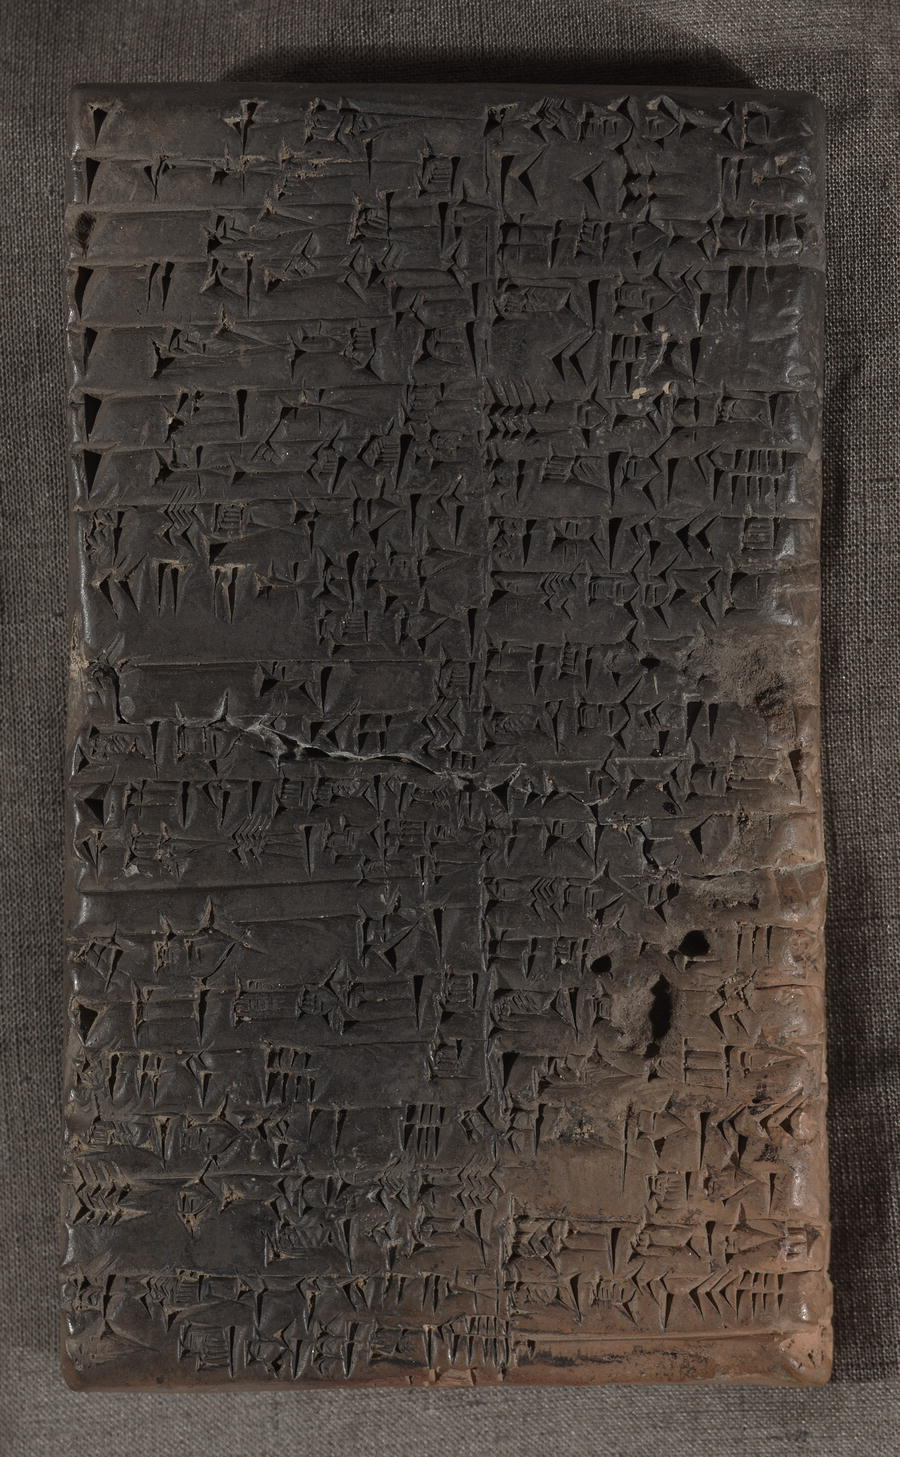
\includegraphics[width=70mm, angle=90]{cuniform_tablet.jpg}
\caption{A cunieform tablet containing ancient payroll information. Amar-Suen. Disbursement of wages. \emph{Cuneiform Tablets: From the Reign of Gudea of Lagash to Shalmanassar III.} Library of Congress, African and Middle Eastern Division, Washington, D.C. 20540. 2039 BCE. http://memory.loc.gov/cgi-bin/query/h?intldl/cunei:@FIELD(DOCID+@BAND(@lit(amcune000013)))}
\end{figure}

Headrick constructs a useful schema for discussing various forms of information technology and gives examples for each: organizing, transforming, displaying, storing, communicating.  He notes certain examples to explore each of these more abstract ways in which we have been working with information from the Enlightenment forward. He covers from the systematization of scientific language with the modern names for chemistry, botany, the inception of the periodic table, through to the telegraph system. My interest here is to draw a throughline between the ideal systems being constructed during this time and the real systems that we are living with today. Many of the basic ways with which we interact with information has remained truly unchanged from the structures we created during the Enlightenment  and Scientific Revolution. We still display data on Cartesian coordinate systems in maps and graphs and still often store sorted data as we have in Dictionaries and Encyclopedias for hundreds of years. On the foundation of these information systems lie the structures we currently have surrounding the complex issues of Intellectual Property.\footnote{Headrick, Daniel. \emph{When Information Came of Age.} (New York : Oxford University Press. 2000) pg.}

\begin{figure}[ht!]
\center
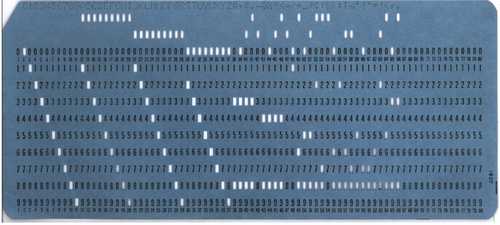
\includegraphics[width=90mm]{500px-Blue-punch-card-front-horiz.png}
\caption{An 80-column punched card of the type most widely used in the 20th century. Card size was 7 3⁄8 in × 3 1⁄4 in (187.325 mm × 82.55 mm). This example displays the 1964 EBCDIC character set, which added more special characters to earlier encodings. Wikimedia foundation. (http://en.wikipedia.org/wiki/Punched\_card) }
\end{figure}

Something something information systems reflecting structures of earlier orgainzational principlles. Relational Databases are like citations, cross references, dictionaries, encyclopedias, etc.

\section{A Revolution or a Monastary}

In the beginning, there were switches.

The Computer Revolution, The Digital Revolution, the Dawning of the Computer Age, or the Dawning of the Age of Aquarius, whatever you want to call it, it happened. The main thrust of this change has already happened. People already take streaming video to handheld devices for granted. It's over folks, we can all go home. Not quite, because there are still a lot of unanswered questions here about how exactly, in less than a generation, we came to create a never before seen communications network that can seamlessly translate transmissions to a variety of protocols, a variety of media, to a worldwide public sphere as envisioned by German critical social theorist Habermas\footnote{Habermas, Jurgen. \emph{The Public Sphere.} New German Critique 3. 1974. pg.}. \footnote{Habermas, Post National Constellation}

The Industrial Revolution brought people to the cities. It built new modes and methods of work, and changed the dynamics of western society.

"The hacker ethic is shorthand for a list of tenets, and it includes a mix of aesthetic and pragmatic imperatives: a commitment to information freedom, a mistrust of authority, a heightened dedication to meritocracy, and the firm belief that computers can be the basis for beauty and a better world."\footnote{Coleman, Gabriela. \emph{Coding Freedom.} 17.} \footnote{Levy, Steven.\emph{Hackers: Heroes of the Computer Revolution.} Durham: Anchor Press/Doubleday. 1984.}

The formation of new academic disciplines has been a regular event over the past two hundred years or so. Various founders of new systematized conceptions for knowledge formation.

Hacking is an intuitive discipline. The language of computing is not English, so translating your ideas into an academic paper does not help to actually construct the forms and programs that actually get things done on the boxes. Formalized computer science attempts to translate the structures and patterns of binary data into english-language equivalents so as to describe them to people who do not have that kind of direct experience. Hackers often eschew the formalized tradition.
\section{Homebrew Clubs to Underground, Emergent}

1970s Counter Culture Outlook Hazy, Computer Clubs

\begin{figure}[ht!]
\center
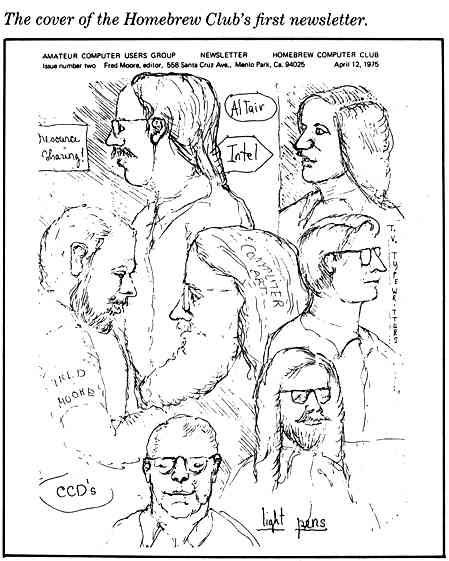
\includegraphics[width=90mm]{homebrew_cover.jpg}
\caption{woz thing that I fucking deleted goddamnit)}
\end{figure}

\begin{verbatim}
PRINT "HELLO WORLD!"
\end{verbatim}
All new programmers will undoubtedly run into some variation of this simple program that allows you to demonstrate basic input output facilities of your machine. The version you see above is BASIC, one of the first consumer-grade languages.

1984 The Archive Begins\footnote{"The Constitution of a Hacker." \emph{2600 Magazine.} March 1984. V1 3}

DoD Funding Repeated

Information should be free

Ostensibly published out of The Metal Shop BBS in Missouri, Phrack Magazine is an underground e-zine, some might say the underground e-zine that transmitted the 
\begin{quote}
Here is what MAXFIELD says, "You got the hackers, and then you got the
people who want to make money off the hackers." Information shouldn't
be free, you should find out things on your own.\footnote{Knight Lightning. \emph{Phrack World News.} Issue XV: Part One -  July 27, 1986}

\end{quote}

15 issues (two years of publishing) until the truism is even mentioned. So ingrained in the culture that it doesn’t even need to be stated explicitly.
\begin{quote}Knowledge is the key to the future and it is FREE. The telecommunications and
security industries can no longer withhold the right to learn, the right to
explore, or the right to have knowledge. The new age is here and with the use
of every *LEGAL* means available, the youth of today will be able to teach the
youth of tomorrow.\footnote{Knight Lightning.\emph{ Phrack World News.} Issue XVIV/1. 1988. Digital.}\end{quote}

Hackers even began noticing their community being discussed by academics, and went as far as to publish copies of papers about them in their zines.

\begin{quote}Levy (1984) and Landreth (1985) both note that some computer aficionados have
developed a "hacker ethic" allowing harmless computer exploration, including
free access to files belonging to other users, bypassing passwords and security
systems, outwitting bureaucrats preventing access, and opposing private
software and copy protection schemes\footnote{Hollinger, Richard C. Computer Hackers Follof A Guttman-Like Progression 1988 Phrack Magazine 2.22 File 7 of 12. Digital.}\end{quote}

The media myth of the Teenage Hacker. It was all bullshit. The problem wasn't that there were a legion of genius hackers, the problem was that there was almost nonexistent security in place, even at the highest levels. Sure, a very small minority of the hackers out there could cause minor trouble on the systems that they had access to...  blarg.

The Hacker Ethic, and the generation of a culture surrounding computers is a somewhat artificial thing. Which is appropriate, considering it's a culture whose primary purpose is engagement and interaction with the current pinnacle of artifice. The conspiracy theorist in me wants to argue that it was an intentionally created thing, a seeded countercultural millieu that trained a legion of teenagers in the bread-and-butter of espionage and spycraft. The ones who get caught aren't necessarily technical wizards. Often those technical wizards who crafted the exploits and wrote the viruses passed them along via an anonymous BBS upload. It's the difference between the people who designed Legos, and the kids who put them together. Different leagues all together.

phone phreaks being that which the media pounced upon, going as far as to label Kevin Mitnick as the John Dillinger of cyberspace.

\section{GNU, GPL, Linux, F/OSS}

Doomsday was a button press away.

The Internet is a system that was designed to survive the Apocalypse. Abstract away the loss of a city. A simple node going down, but the network, and therefore, the nation, civilization, humanity, survives.

The laws that we have in place now were created during this time when a Revolution meant bowing to an outside power. The Communist threat...  Hackers were enemies, domestic. They were able to subvert everything that held the social order together.

The systems intended purpose was to implement military command and control. The money and resources that we pour into them are an unofficial taxation for systems that need to exist to keep the power structures functioning.

It takes power to feed the people that build and maintain the networks, to keep them building, to keep them maintaining. Hackers can, and often do, get a free ride. They can do things with these machines that others cannot. With the explosion of the consumer computer revoluton pushed by those monetizing the technology....  The gulf between those who use, and those who design, has widened over the past 40 years.

Science Fiction movies and television have become future marketing for the imaginations twenty years down the line.

Radio transmitters the size of postage stamps embedded in computers more powerful than any of the original hackers imagined can transmit encyclopedias worth of data over the course of hours or minutes.

Billions of switches. Switches nested on top of switches. An infinite russian doll of ones and zeroes.

PACKET AND HAM RADIO

Information transmission over time.

The court of empire, but no emperor.

Fragmented power...  creates tension...

multiple tension

military, domestic government, finance

Computer liberate us

Post cold war ideology?

Stuck in cold-war ideology.

The cold war never ended.

The participants changed.

Ecosystems on earth only survive because of the constant oppressive power of the sun flooding into them.

Society creates false utopias.

J. Forrester - Early Warning Network
Feedback Loops

Out there thesis: The hacker culture as an underground was intentionally created in order to train a multitude in the lifestyle of the intelligence and security communities.

Examine the commonalities between the double lives led by computer criminals, and intelligence officers.

Cold War society engineering.

Networks are means by which people can communicate useful information

What information is pulled?

Holistic vision of networked systems.

Hackers as codebreakers,
digital gypsies,
disambiguation of piratical personages

roguish talents can save the day in the right context.

\footnote{Abbate, Janet. "Cold war and white heat: the origins and meanings of packet switching." in \emph{The social shaping of technology 1999,} ed. Donald A MacKenzie and Judy Wajcman.Philadelphia: Open University Press. 1999. Print. 351.}

Isn't it better to have teenagers with curious intent break into your military and industrial computer systems rather than letting those vulnerabilities remain until a determined and malicious attacker appears?

\section{Conclusion}



The progressive conceit that we hold since the Enlightenment is a thin veneer on top of the archetypal mythic cycles that underly our metaphorical ontology.  The mythic Hacker is yet another manifestation of this archetypal western genius, starting from Archimedes, going on through Newton et al.  They are all Nietzsche’s madman, each one of these historical personas are another manifestation of this same central character, popular past the point of cliche. As in Nietzsche’s classic Parable of the Madman, they shine on the field of knowledge with their own lantern, even though to everyone else it seems bright as noon. Nietzsche’s madman famously yelled, “God is dead!” Hackers are portrayed as ubermench ultra-genius philospher-kings, able to see past the dancing shadows on the screen to the truth of the bits and bytes behind the curtain.

Well, it’s about time that we slay the myth of the Hacker Trickster-god, because it’s bamboozling a generation. It’s inverting the mode of the bizairre social effects as being a side effect of what psychologists might label as socially maladaptive obsessive behavior. In fact, there were early writings pointing at the early hackers as “obsessive computer programmers.” (Weizenbaum, Computer Power and Human Reason, 1975) These bizairre social effects are the only parts that the outsider can witness, because so much of the real work is done with mental constructs and the structures that create the finished products. I will be using the terminology of Hackers and Hacker culture in erasure. I will use these words in order to access the full connotations that they suggest, but also reject these connotations.

There is so much that has been written about open source software that it is absolutely impossible to keep up with everything. Especially if we want to start to delve into code as an artifact to be studied. That would be outside of the scope of this project.  I am going to be looking to a number of texts, written by hackers, as primary sources. I will also be pointing to a growing body of recently conducted scholarship in Anthropology to support my assertion that the People of the Internet are an indigenous culture to the virtual space in the networks. I will argue that this People of the Internet has been slowly networking and growing as a global indigenous culture.

This writer is speaking as one of those bodies who was standing on the ground outside of the first Anonymous protests against Scientology. This writer is speaking as one of those who was watching in Zuccotti, and Oakland, and Seattle, and Houston, and Tahrir. This writer is speaking as one of those who was watching via live-stream outside of the Argentinian Embassy as Julian Assange waited for the statement by the Argentinian President regarding his assylum. I am not speaking as an outside academic observer who spent some time embedded in this culture in order to study “geeks” like they were some kind of lost Amazon tribe. Think of me as the Thucydidies of Cyberspace.

Today, we’re seeing this culture hitting a new stage in it's evolution, the first hackers having birthed children who have come of majority, some of which have taken up the Hacker banner themselves. Hackers bred, at least those who could operate outside of their all-consuming obsession for the machine, those who could battle thi madness for long enough to nurture relationships, those who swore to hold back from the absolute abyss, those who weren’t consumed in the fires of their creation. They transmitted, whether via explicit instruction or implicitly through behavior modeling, the hacker behaviors that created the new wave of computer hackers.  While there was a massive amount of media attention directed toward this relatively minor criminal element, there was another culture arising. While the engineers of the internet were attempting to solve the technical problems of the original Internet. BBS users built a grassroots parallell network that stands to this day. Much of the cultural conventions that are on the internet today were born out of the BBS community.

Now we need to explore the idea that ideas evolving in an ecosystem, hybridizing, breeding, growing, and some dying out. And, we also need to explore ideational convergent evolution. As it so happens, like Newton and Leibniz both seem to have independently invented the mathematical ideas that we so rudely codify into Calculus textbooks, many of these ideas were developed by different people in different places, independent of the other. So should the legitimacy of simple ideas be defined by a race to the patent office? Who gets the global rights to an algorithm that is probably actually already encoded in some dead mathematician’s notes? This is a can of worms that I will not be opening in this paper, except maybe to get a little whiff of the problem. It doesn’t smell very appetizing, but it will be necessary to settle the Intellectual Property debate in the future.

I'm snagging up likely sources/citations and popping them here at the end.

\footnote{Nelson, Ted. \emph{Computer Lib}. Self. 1974.}

\footnote{Johns, Adrian. \emph{Piracy: The Intellectual Property Wars from Gutenberg to Gates}. Univ of Chicago Press. 2010. Print.}

\footnote{Ceruzzi, Paul E.\emph{A History of Modern Computing.}}

\footnote{Firstname Lastname, Title of Book. Place of  publication: Publisher, Year of publication.}

\end{document}